\documentclass{article}
\usepackage{graphicx}

\begin{document}

\begin{center}


\includegraphics[width=3cm]{IMG_20260310_120019.jpg}

\vspace{0.5cm}

{\huge Gate Logic Circuit Analysis}

\vspace{0.3cm}

Keshava Reddy V

ID: COMETFWC054

\end{center}

\section*{Question}

For any set of inputs $A$ and $B$, the following circuits give the same output $Q$, except one.

Which one is it? (GATE PH 2010)

\section*{Analysis}

We simplify each circuit using Boolean algebra.

Option (b):

$Q = A \cdot \overline{B}$

Option (c):

$Q = A \cdot \overline{B}$

Option (d):

$Q = \overline{A} + B$

Hence option (d) gives a different output.

\section*{Python Code}

\begin{verbatim}
import numpy as np
import matplotlib.pyplot as plt

A = np.array([0,0,1,1])
B = np.array([0,1,0,1])

Qa = (A ^ B) & (~B & 1)
Qb = A & (~B & 1)
Qc = (A & (~B & 1)) | ((~A & 1) & B)
Qd = (~A & 1) | B
\end{verbatim}

\section*{Graph}

\begin{center}

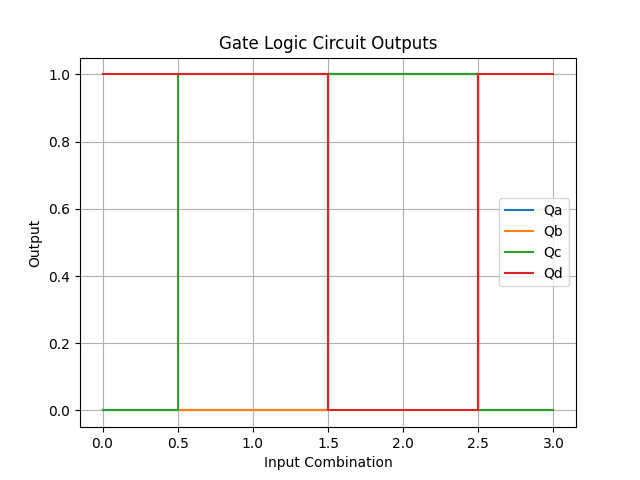
\includegraphics[width=10cm]{q41_graph.png}

\end{center}

\section*{Conclusion}

Options (b) and (c) produce the same Boolean expression.

Option (d) gives a different output.

Therefore the correct answer is option (d).

\end{document}
